\paragraph{$R_0$ definition}
%
The basic reproductive number, which is generally denoted by $ R_0 $,
is a threshold quantity with which we can use 
particular control strategies. The epidemiological interpretation of 
$ R_0 $ is the average number of secondary cases produced by an infected
individual introduced into a population of susceptible individuals.
Using Van DenDrishe's \cite{VandenDriessche2017a} definition of reproductive number
we obtain
\begin{equation*}
    \label{eqn:reproductive_number}
    \begin{aligned}
        R_0 :=
        &
        \frac{\kappa}{(\kappa + \mu)(\delta_L + \mu)}
        \left(
            \mu R_1 + \delta_L
        \right)
        \left[
            \frac{p\beta_S}{R_2}
            +\frac{(1 - p) \beta_A}{\gamma_A+\mu}
        \right],
    \\
    \text{where} &
    \\
        R_1 &= 1 - \theta(1 - \epsilon),
    \\
        R_2 &= \mu + \delta_H + \gamma_S + \mu_{I_{S}}.
    \end{aligned}
\end{equation*}
%
The factor $\frac{p\beta_S}{R_2}$ measures the proportion of new infections
generated by a symptomatic infectious individual in the time that it lasts
infected. In a similar way, the factor $\frac{(1 - p) \beta_A}{\gamma_A+\mu}$
measures the new infections generated by an asymptomatic infectious individual
in the time that it lasts infected. The factor 
$\frac{\mu R_1 + \delta_L}{\delta_L + \mu}$ measures the number
of individuals in lockdown that leave the lockdown, which can be infected.
And finally, the factor $\frac{\kappa}{\kappa + \mu}$ measures
the time of the disease's incubation.
%
If we consider that there is no lockdown, we have that $ R_0 $ is reduced to
\begin{equation*}
    \label{eqn:reproductive_number}
    \begin{aligned}
        \tilde{R}_0 :=
        &
        \frac{\kappa}{(\kappa + \mu)}
        \left[
            \frac{p\beta_S}{R_2}
            +\frac{(1 - p) \beta_A}{\gamma_A+\mu}
        \right].
    \end{aligned}
\end{equation*}
%
Note that we have the relation $ R_0 \leq \tilde{R}_0 $. These indicate that there is greater transmission of the disease if there is no lockdown.

\paragraph{No  vaccine reproductive number}
\paragraph{Vaccine reproductive number}
\paragraph{Efficacy, coverage and vaccination rate}

\comment[id=SDIV]{%
    Here countor plots figure as function of efficacy and
    vaccination rate%
}
%
\added[id=SDIV]{Here Gabriel's R not calculations.}
%
Considering assumptions 2, we can establish a vaccine reproductive number,
in which individuals who have already been vaccinated
can become infected individuals by being in contact with the
symptomatic infected. Using Van den Driessche’s \cite{VandenDriessche2017a}
definition of reproductive number and \cite{Alexander2004}, we obtain

\begin{equation*}
 R_{0}^V := \left[ 1-\frac{\varepsilon \lambda_V}
 {\mu+\lambda_V+\delta_V}
 -\frac{\theta\mu(1-\epsilon)}{\mu+\delta_L+\lambda_V}\right]
 (\mu R_1+\delta_L)R_0.
\end{equation*}
%
The threshold quantity $R_0^V$ is the reproductive number of infection
which can be interpreted as the number of infected people produced
by one infected individual introduced into the population in the
presence of vaccination.

\comment{edit plot range to display level RV=1}
\begin{figure*}[tbh]
    \centering
      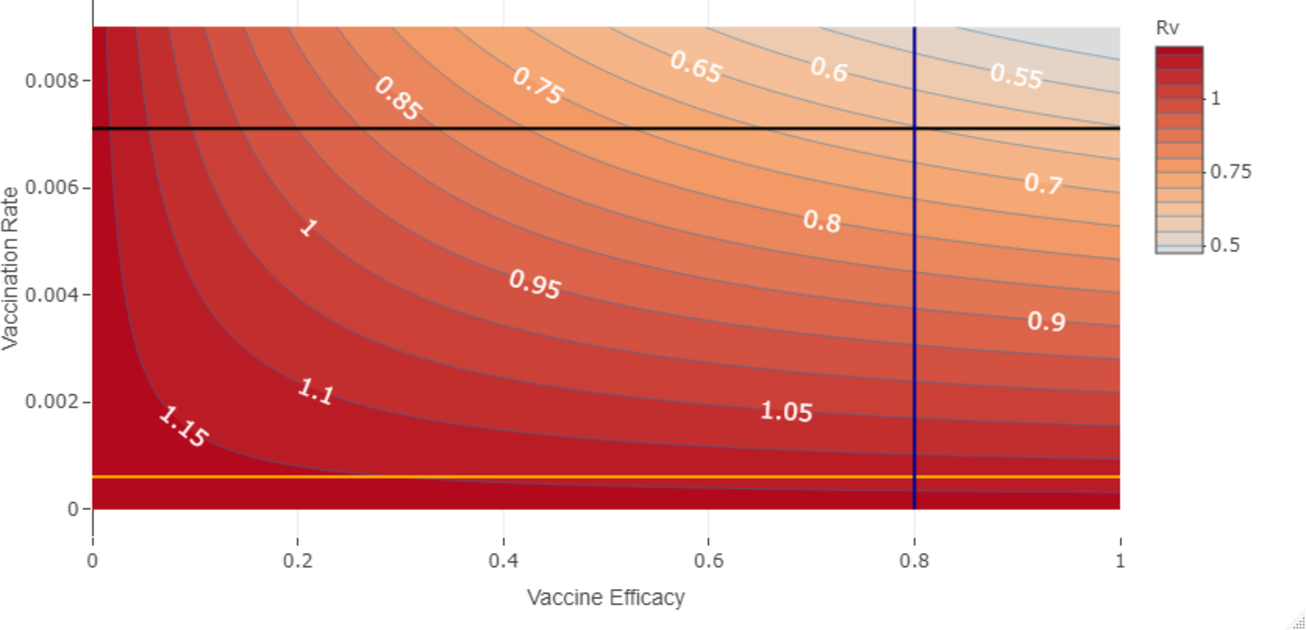
\includegraphics[scale=0.5, keepaspectratio]{Figures/Rv_contour}
    \caption{R not contour plot as function of efficacy and vaccination rate.}
    \label{fig:rvcontour1}
\end{figure*}
\begin{figure*}[tbh]
    \centering
      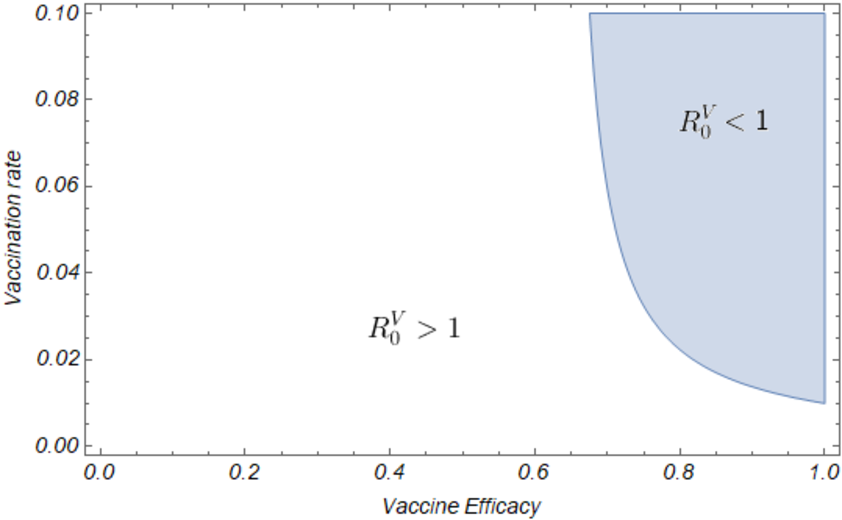
\includegraphics[scale=0.7, keepaspectratio]{COVID19-VACINATION/Figures/No-Lockdown-Vaccination.pdf}
    \caption{No lockdown Region $R_v<1$.
    \href{https://plotly.com/~AdrianSalcedo/52/}{%
		https://plotly.com/~AdrianSalcedo/52/}
    }
    \label{fig:Nolockdown}
\end{figure*}

\begin{figure*}[tbh]
    \centering
      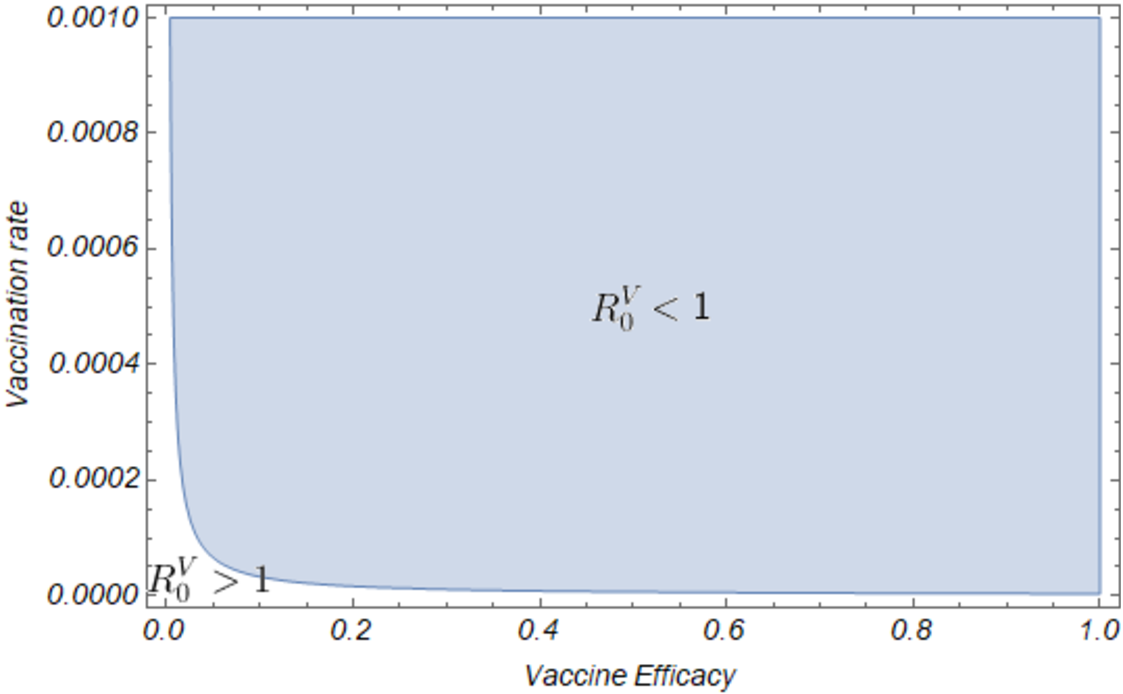
\includegraphics[scale=0.7, keepaspectratio]{COVID19-VACINATION/Figures/Lockdown-Vaccination.pdf}
    \caption{lockdown Region $R_v<1$.
        \href{https://plotly.com/~AdrianSalcedo/54/}{%
		https://plotly.com/~AdrianSalcedo/54/}
    }
    \label{fig:Lockdown}
\end{figure*}